\chapter{Kiến thức nền tảng}
\section{Công nghệ đã được sử dụng}
\subsection*{PyTorch}
\subsection*{Jupyter Notebook và Google Colab}
\section{Những mô hình học sâu nền tảng}
\subsection{Mạng thần kinh nhân tạo - Artificial Neural Network}
Mạng thần kinh nhân tạo là một hướng đi trong lĩnh vực học máy, với nguồn cảm hứng được lấy từ tính kết nối của các neuron thần kinh trong bộ não sinh vật.

Đơn vị nhỏ nhất cấu tạo nên một mạng thần kinh nhân tạo sẽ là một neuron nhân tạo, hay còn được biết đến là một Perceptron. Các Perceptron sẽ được sắp xếp thành từng lớp, với luồng dữ liệu đi từ những neuron ở lớp trước sang lớp sau. Hai neuron được nối với nhau có thể truyền tải dữ liệu cho nhau, mô phỏng lại việc truyền tín hiệu giữa các synap thần kinh.

Mạng thần kinh nhân tạo phụ thuộc vào dữ liệu đã được xử lý sẵn để tự huấn luyện, cải thiện độ chính xác của bản thân. Quá trình tự huấn luyện sẽ giúp mạng phát hiện được những quy luật bên trong dữ liệu mà không cần sự can thiệp của con người. Vì vậy nên, những mô hình này có thể phát hiện ra được những quy luật chính xác hơn và hiệu quả hơn so với những quy luật được định nghĩa thủ công bởi chuyên gia.
\subsubsection*{Perceptron}
Perceptron là một thuật toán giúp phân loại dữ liệu theo hai lớp. Perceptron sẽ nhận vào một số lượng bất kỳ dữ liệu, áp dụng các trọng số được gán với mỗi dữ liệu đầu vào và một giá trị dời để tạo thành một hàm tuyến tính. Sau đó, kết quả của hàm tuyến tính sẽ được đi qua một lớp kích hoạt, đưa giá trị này về một trong hai phân loại đã được định nghĩa bằng đầu dựa vào một giới hạn đã được định trước(thường là giá trị 0).

Phương thức hoạt động của một Perceptron có thể được thể hiện qua công thức
$$
  f(X) = \Theta(w\cdot X + b)
$$
\[
  \Theta(x) =
  \begin{cases}
    1 & \text{if $x>=0$} \\
    0 & \text{if $x<0$}
  \end{cases}
\]

Tuy nhiên, một vấn đề của mô hình Perceptron là mô hình sẽ chỉ xử lý tốt với những dạng dữ liệu có thể phân tách được ở dạng tuyến tính và chỉ hoạt động được với hai lớp phân loại do hàm kích hoạt. Vì vậy nên, để có thể mô hình hóa được những dạng dữ liệu có cấu trúc phức tạp hơn, nhiều mô hình Perceptron sẽ được kết hợp lại với nhau để tạo thành mạng Perceptron nhiều lớp.
\begin{figure}[H]
  \centering
  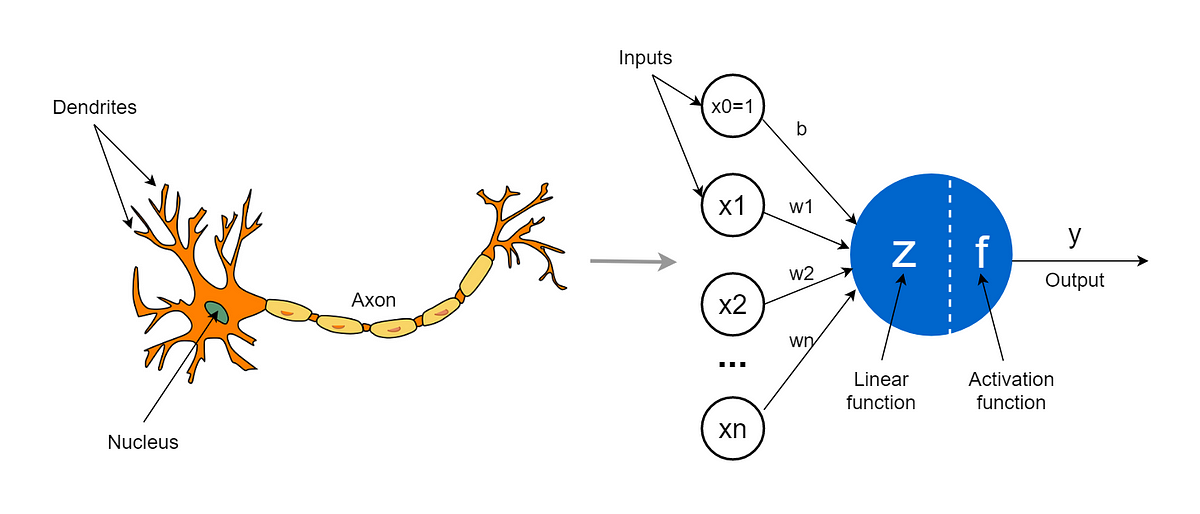
\includegraphics[scale=0.3]{pics/Chapter3/bioNN.png}
  \caption{Synap thần kinh là đơn vị cơ bản của hệ thống thần kinh và là nguồn cảm hứng để ứng dụng Perceptron vào lĩnh vực học sâu \cite{abraham2005artificial}}
  \label{fig:enter-label}
\end{figure}

\subsubsection*{Mạng Perceptron nhiều lớp}
Đây là một cấu trúc cơ bản, một ví dụ điển hình của mạng thần kinh nhân tạo với đơn vị nhỏ nhất là các Perceptron. Mạng này sẽ được cấu tạo từ nhiều lớp khác nhau, mỗi lớp sẽ bao gồm các Perceptron có đầu vào là những Perceptron ở lớp trước và đầu ra sẽ được nối vào Perceptron ở lớp sau.

Tín hiệu, là những số thực, sẽ được truyền từ Perceptron ở lớp trước sang Perceptron của những lớp sau qua các cạnh liên kết. Mỗi cạnh sẽ được gán một trọng số. Trọng số này sẽ quyết định mức độ quan trọng của tín hiệu đi qua cạnh liên kết đó. Trong quá trình xử lý, các tín hiệu qua mỗi cạnh sẽ được nhân với trọng số tương ứng và cộng với lại độ dời ở nút Perceptron. Sau đó, kết quả này sẽ được đi qua một lớp phi tuyến tính để có thể thích ứng với nhiều kiểu dữ liệu khác nhau, không như một Perceptron đơn giản.
\begin{figure}[H]
  \centering
  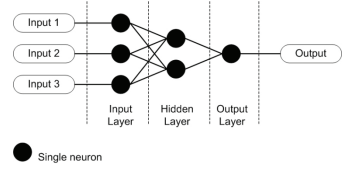
\includegraphics{pics/Chapter3/basicNN.png}
  \caption{Cấu tạo của một mạng neuron nhân tạo cơ bản \cite{krenker2011introduction}}
  \label{fig:enter-label}
\end{figure}
\subsubsection*{Huấn luyện mạng neuron}
Quá trình học hỏi của một mạng neuron nhân tạo cơ bản sẽ xuất phát từ việc xác định kết quả ban đầu từ dữ liệu đầu vào, tính ra sai số giữa kết quả của mô hình và kết quả đúng được cung cấp. Sau đó, mô hình sẽ điều chỉnh lại các trọng số bên trong mô hình để giảm thiểu sai số đó. Qua mỗi lần điều chỉnh, kết quả đầu ra của mô hình sẽ càng trở nên giống với kết quả đúng hơn. Khi đạt đến một ngưỡng nhất định, việc huấn luyện sẽ được ngừng lại để ngăn việc kết quả của mô hình quá phụ thuộc vào tập dữ liệu.

Cơ chế điều chỉnh trọng số này được gọi là cơ chế truyền ngược. Cụ thể hơn, cơ chế này sẽ được thực hiện thông qua các bước
\begin{enumerate}
  \item Tính toán sai số giữa kết quả đầu ra của mô hình và kết quả thực.
  \item Đối với mỗi trọng số ở lớp cuối cùng, giá trị đạo hàm dựa trên sai số có thể tính được không quá khó khăn. Một bội âm của mỗi giá trị đạo hàm sẽ được dùng để điều chỉnh trọng số, nhằm hướng đến việc đạt đến sai số tối thiểu.
  \item Bước 2 sẽ được lần lượt thực hiện, đi từ lớp gần cuối tới lớp đầu tiên của mô hình. Giá trị đạo hàm tại mỗi lớp sẽ được tính dựa trên lớp ngay sau đó bằng quy tắc dây chuyền của Leibniz trong việc tính đạo hàm.
\end{enumerate}

\begin{figure}[H]
  \centering
  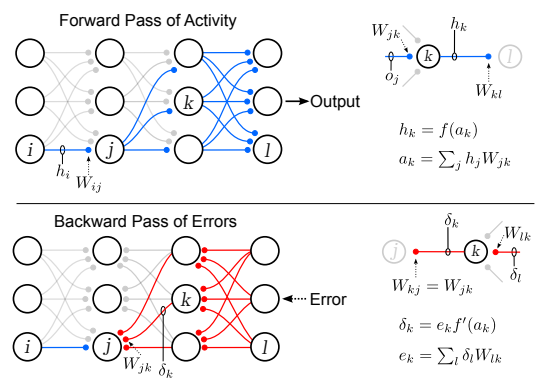
\includegraphics{pics/Chapter3/backprop.png}
  \caption{Biểu đồ mô phỏng quá trình thực hiện cơ chế truyền ngược ở một mạng neuron đơn giản \cite{lillicrap2020backpropagation}}
  \label{fig:enter-label}
\end{figure}

\subsection{Mạng neuron tích chập - Convolutional Neural Network}
\subsubsection*{Định nghĩa}
Mạng neuron tích chập, hay còn được gọi là CNN hay ConvNet, là một loại mạng neuron nhân tạo được thiết kế để xử lý những dạng dữ liệu có cấu trúc dạng bảng, như một hình ảnh. Trong máy tính, hình ảnh sẽ được lưu dưới dạng một bảng các điểm ảnh, với mỗi điểm ảnh chứa các dữ liệu nhằm thể hiện màu sắc và độ sáng của điểm ảnh đó.


Mạng neuron tích chập sẽ giúp tối ưu hóa quá trình huấn luyện mô hình trên một lượng lớn dữ liệu ở dạng bảng. Cụ thể hơn, để huấn luyện một lớp của mạng neuron nhân tạo truyền thống, là một mạng kết nối đầy đủ giữa các lớp, trên một ảnh có kích thước $100x100$ điểm ảnh, 10000 trọng số sẽ cần được sử dụng và điều chỉnh trong quá trình huấn luyện. Việc sử dụng một số lượng lớn trọng số sẽ gây ra các vấn đề về tài nguyên tính toán, cũng như việc áp dụng cơ chế truyền ngược - làm cho giá trị đạo hàm bị tăng không kiểm soát hoặc biến mất.

Tuy nhiên, nhờ vào việc áp dụng các bộ lọc trong những lớp tích chập, số lượng trọng số cần được xử lý sẽ giảm đi một cách đáng kể. Một ảnh có độ phân giải $100x100$ vẫn có thể được giải quyết bằng một bộ lọc $5x5$, với 25 trọng số. Kết quả đầu ra vẫn sẽ giữ cấu trúc dạng bảng, và những bảng giá trị ở những lớp càng nằm ở phía sau sẽ càng chứa nhiều thông tin từ bức ảnh, mà không tiêu tốn quá nhiều tài nguyên tính toán, cũng như né được những vấn đề liên quan đến cơ chế truyền ngược bằng đạo hàm.
\begin{figure}[H]
  \centering
  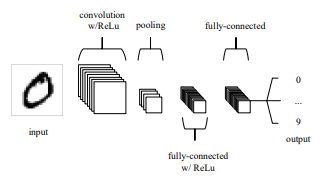
\includegraphics{pics/Chapter3/conv_kernel2.png}
  \caption{Một mạng neuron tích chập cơ bản \cite{o2015introduction}}
  \label{fig:enter-label}
\end{figure}
Mạng neuron tích chập được lấy cảm hứng từ cách mà bộ não con người xử lý hình ảnh thu nhận được từ mắt.  Mỗi neuron sẽ hoạt động dưới một lớp tế bào cảm thụ ánh sáng riêng và các neuron sẽ được nối với những neuron ở những lớp khác để có thể bao phủ được toàn bộ vùng võng mạc ở mắt. Tương tự như cách mà mỗi phần của một bức ảnh sẽ được xử lý ở những vùng trên võng mạc mắt, các bộ lọc của mạng neuron tích chập cũng sẽ chạy và xử lý từng mảng nhỏ của bức ảnh. Qua các lớp, những chi tiết được phát hiện sẽ tăng dần về độ phức tạp, từ những chi tiết đơn giản như cạnh, đường cong,... và tăng dần đến những chi tiết phức tạp như khuôn mặt, đồ vật,... Nói cách khác, mạng neuron tích chập đã cho các mô hình học máy khả năng xử lý ảnh của mắt người.

\subsubsection*{Lớp tích chập}
Lớp tích chập là một lớp trích xuất đặc trưng ở dữ liệu đầu vào và bảo toàn mối quan hệ giữa các điểm ảnh. Lớp tích chập sẽ nhận vào một tập các điểm ảnh có dạng bảng, có cấu tạo là $HxWxC$ với H là độ cao, W là độ rộng và C là số kênh dữ liệu có trong ảnh. Ban đầu, H và W sẽ phụ thuộc vào độ phân giải của ảnh và các ảnh thông thường sẽ gồm 3 kênh dữ liệu, đại diện cho 3 màu RGB.


Sau đó, ở bên trong lớp tích chập, một hay nhiều bộ lọc sẽ được trượt trên tất cả các mảng của ảnh. Tại mỗi mảng được một bộ lọc trượt qua, phép toán nhân ma trận Frobenius sẽ được sử dụng để tính ra một giá trị mã hóa cho chi tiết tại mảng đó. Công thức của phép toán nhân ma trận Frobenius được thể hiện như sau.

Với ma trận $A$ và $B$ được thể hiện như bên dưới,
$$
  {\displaystyle \mathbf {A} ={\begin{pmatrix}A_{11}&A_{12}&\cdots &A_{1m}\\A_{21}&A_{22}&\cdots &A_{2m}\\\vdots &\vdots &\ddots &\vdots \\A_{n1}&A_{n2}&\cdots &A_{nm}\\\end{pmatrix}}\,,\quad \mathbf {B} ={\begin{pmatrix}B_{11}&B_{12}&\cdots &B_{1m}\\B_{21}&B_{22}&\cdots &B_{2m}\\\vdots &\vdots &\ddots &\vdots \\B_{n1}&B_{n2}&\cdots &B_{nm}\\\end{pmatrix}}}
$$
Giá trị của phép nhân ma trận Forbenius giữa $A$ và $B$ là
$$
  {\displaystyle \langle \mathbf {A} ,\mathbf {B} \rangle _{\mathrm {F} }=\sum _{i,j}{\overline {A_{ij}}}B_{ij}\,=\mathrm {Tr} \left({\overline {\mathbf {A} ^{T}}}\mathbf {B} \right)\equiv \mathrm {Tr} \left(\mathbf {A} ^{\!\dagger }\mathbf {B} \right)}
$$
với ký hiệu gạch đầu là phép tính số phức liên hợp và ký hiệu $\!\dagger$ thể hiện phép nghịch đảo ma trận và tính số phức liên hợp trên tất cả các phần tử. Tuy nhiên, do lớp tích chập chỉ xử lý dữ liệu các số thực, cho nên công thức có thể được đơn giản hóa thành
$$
  {\displaystyle {\begin{aligned}\langle \mathbf {A} ,\mathbf {B} \rangle _{\mathrm {F} }=&{ {A}}_{11}B_{11}+{ {A}}_{12}B_{12}+\cdots +{ {A}}_{1m}B_{1m}\\&+{ {A}}_{21}B_{21}+{ {A}}_{22}B_{22}+\cdots +{ {A}}_{2m}B_{2m}\\&\vdots \\&+{ {A}}_{n1}B_{n1}+{ {A}}_{n2}B_{n2}+\cdots +{ {A}}_{nm}B_{nm}\\\end{aligned}}}
$$

\begin{figure}[H]
  \centering
  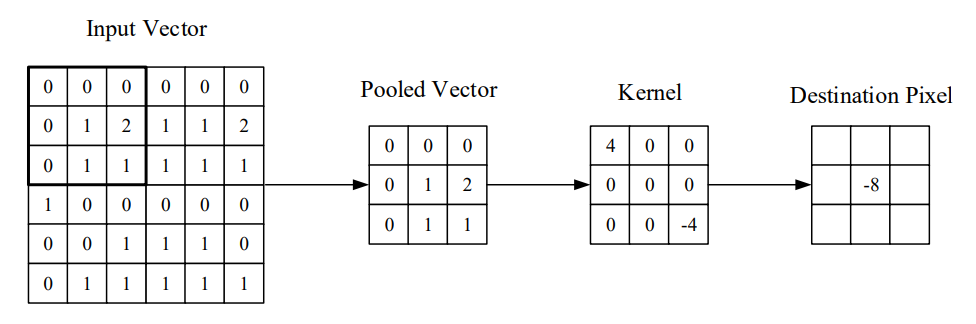
\includegraphics[scale=0.5]{pics/Chapter3/conv_kernel.png}
  \caption{Áp dụng một bộ lọc kích thước $3x3$ lên một mảng của ảnh \cite{o2015introduction}}
  \label{fig:enter-label}
\end{figure}

Sau đó, kết quả sẽ được chạy qua một hàm kích hoạt, thông thường là ReLU để tạo sự phi tuyến tính.

Một số tham số có thể điều chỉnh cho quá trình chạy lớp tích chập chính là kích thước của lớp lọc, bước nhảy, và kích thước phần đệm. Bước nhảy sẽ quy định độ dời về điểm ảnh sau mỗi lần xử lý từng mảng của bộ lọc. Kích thước phần đệm sẽ có tác dụng thay đổi kích thước của dữ liệu đầu vào bằng cách thêm các số 0 dọc theo đường viền của bảng dữ liệu, giúp điều chỉnh ảnh phù hợp với kích thước bộ lọc và bước nhảy. Cuối cùng, kích thước của bộ lọc sẽ quy định độ lớn của mảng được xử lý trong một lần chạy. Trước đây, các bộ lọc có kích thước lớn như $7x7$ sẽ được sử dụng để làm lớp tích chập đầu tiên, nhằm gom cụm lại các chi tiết trên ảnh hiệu quả hơn. Tuy nhiên, qua quá trình phát triển của mạng neuron tích chập, việc sử dụng nhiều bộ lọc có kích thước $3x3$ liên tiếp đã được phát hiện là vẫn sẽ bao phủ được một vùng có kích thước lớn với số trọng số cần điều chỉnh ít hơn. Vì vậy nên, những bộ lọc có kích thước $3x3$ đã trở nên phổ biến trong việc thiết kế mạng neuron tích chập \cite{simonyan2015deep}.


\subsubsection*{Lớp tổng hợp}
Lớp tổng hợp sẽ có tác dụng giúp làm giảm lượng dữ liệu trên bảng khi hình có kích thước quá lớn, mà vẫn giữ được những thông tin quan trọng. Các giá trị tại một mảng sẽ được tổng hợp lại thành một giá trị đại diện sau khi qua lớp tổng hợp. Các phương pháp chính được áp dụng cho lớp tổng hợp bao gồm:
\begin{itemize}
  \item Max pooling: từ mảng đang xét, giá trị lớn nhất sẽ được chọn để đại diện cho cả mảng.
  \item Average pooling: giá trị trung bình của mảng đang xét sẽ được chọn làm đại diện.
\end{itemize}
\begin{figure}[H]
  \centering
  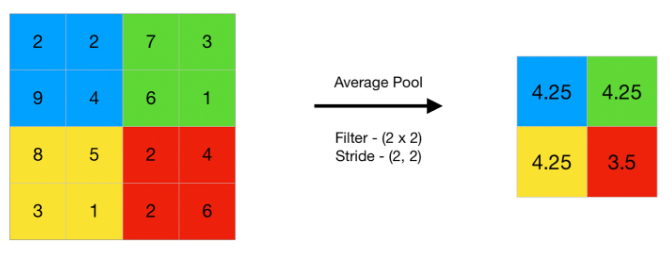
\includegraphics[scale=0.7]{pics/Chapter3/avgpool.png}
  \caption{Lớp tổng hợp sử dụng Average Pooling \cite{poolingg4g}}
  \label{fig:enter-label}
\end{figure}
\begin{figure}[H]
  \centering
  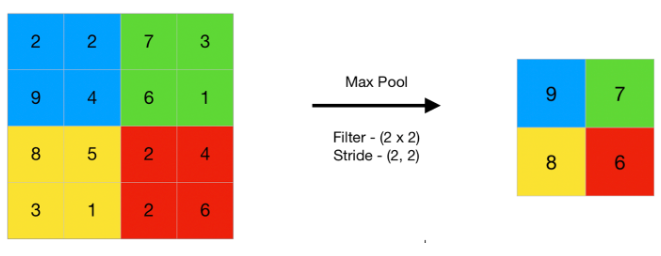
\includegraphics[scale=0.7]{pics/Chapter3/maxpool.png}
  \caption{Lớp tổng hợp sử dụng Max Pooling  \cite{poolingg4g}}
  \label{fig:enter-label}
\end{figure}
\section{Kiến thức về phương pháp nhận diện địa điểm trực quan bằng MixVPR}
Trong bài toán về nhận diện địa điểm trực quan - Visual Place Recognition, đa số các phương pháp có thể được phân vào hai lớp chính, dựa vào vị trí hoặc dựa vào những điểm chung\cite{yin2022general}.
\begin{itemize}
  \item Đối với các phương pháp dựa vào vị trí, một địa điểm đã được đi qua rồi sẽ có thể được nhận biết mà không cần phụ thuộc vào góc nhìn và những điều kiện môi trường xung quanh.
  \item Đối với những phương pháp nhận biết dựa vào điểm chung, thông tin về môi trường xung quanh sẽ được thu lại thông qua ảnh chụp góc nhìn. Từ đó, những phương pháp truy xuất ảnh sẽ được sử dụng nhằm tìm kiếm từ hệ cơ sở dữ liệu một ảnh có độ tương đồng cao.
\end{itemize}
\begin{figure}[H]
  \centering
  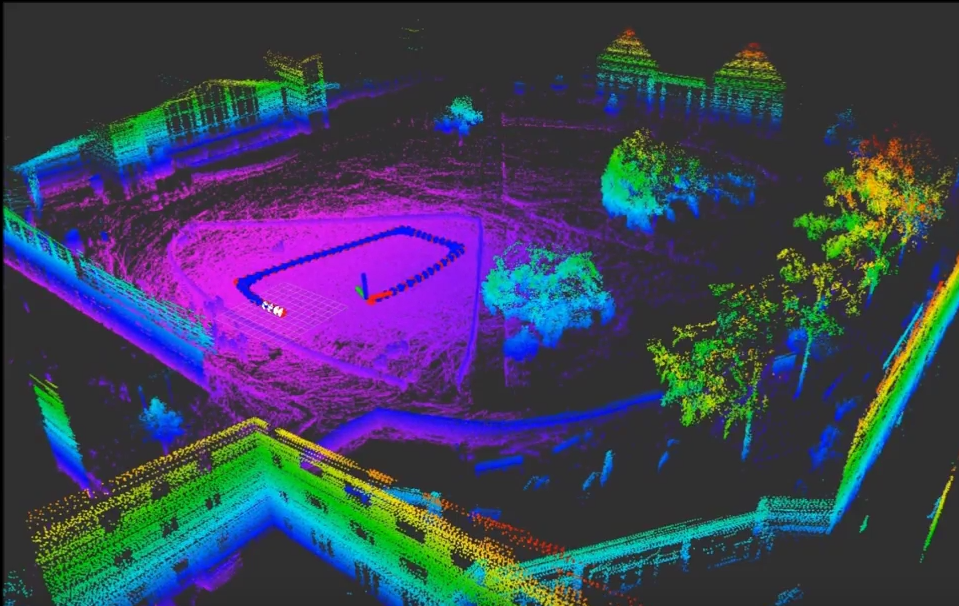
\includegraphics[scale=0.4]{pics/Chapter3/position-based.png}
  \caption{Hình minh họa cho phương pháp nhận diện địa điểm trực quan thông qua những địa điểm đã qua \cite{slamposition}}
  \label{fig:enter-label}
\end{figure}
\begin{figure}[H]
  \centering
  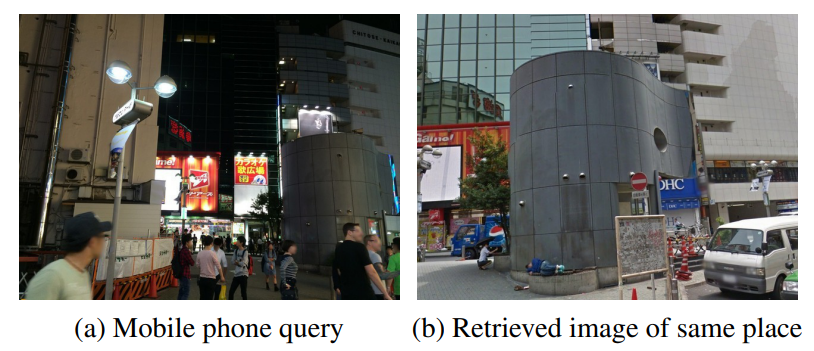
\includegraphics[scale=0.7]{pics/Chapter3/overlap-based.png}
  \caption{Hình minh họa cho phương pháp nhận diện địa điểm trực quan thông qua việc truy xuất ảnh từ hệ cơ sở dữ liệu \cite{arandjelovic2016netvlad}}
  \label{fig:enter-label}
\end{figure}

Mô hình Mix-VPR được chọn là một phương pháp nhận biết dựa vào điểm chung giữa ảnh truy vấn và các ảnh bên trong hệ cơ sở dữ liệu, đại diện cho một khu vực cần được biểu diễn. Mix-VPR so sánh các ảnh với nhau thông qua việc truy xuất đặc trưng của các ảnh và tìm cặp ảnh có đặc trưng mang điểm tương đồng cao nhất.

\subsection{Trích xuất đặc trưng}
Để có thể tìm được những ảnh lân cận, có sẵn tọa độ GPS, những đặc trưng của ảnh sẽ được tạo ra thông qua một quá trính trích xuất và so sánh với lẫn nhau. Phương pháp này hoạt động dựa trên việc những ảnh có góc nhìn, vị trí gần nhau thì sẽ nhìn cùng một tập hợp các vật thể, dẫn đến việc ảnh sẽ có những chi tiết bị trùng lặp ở các vật thể đó. Tuy nhiên, việc chỉ so sánh ảnh với nhau ở mức độ từng điểm ảnh sẽ tạo ra một lượng dữ liệu rất lớn và có thể không cần thiết.

Vì vậy nên việc sản sinh ra các đặc trưng cho hình ảnh sẽ giúp mã hóa ảnh một cách tối ưu mà không làm mất những thông tin quan trọng trong hình. Qua thời gian, việc trích xuất đặc trưng trong lĩnh vực nhận diện địa điểm trực quan(Visual Place Recognition) đã có những bước phát triển nhất định, từ việc chỉ trích xuất những đặc trưng cục bộ trong ảnh. Sau đó, một lớp tổng hợp các đặc trưng cục bộ sẽ được sử dụng \cite{pion2020benchmarking}. Cuối cùng, với sự phát triển của các mô hình học sâu, mạng neuron tích chập đã được huấn luyện để có thể tạo thành những đặc trưng toàn cục của ảnh từ bản đồ đặc trưng đạt được từ những lớp tích chập của mạng.
\subsubsection*{Đặc trưng cục bộ}
Quá trình trích xuất đặc trưng cục bộ sẽ bao gồm hai bước là xác định những yếu tố trọng tâm trong ảnh và xây dựng những đặc trưng xung quanh những yếu tố đó. Trong trường hợp lý tưởng, kết quả đầu ra sẽ là những đặc trưng cục bộ tương đồng dưới những điều kiện khác nhau như thay đổi độ sáng, tỷ lệ hình ảnh, độ nhiễu ảnh, cũng như những góc quay khác nhau \cite{lowe1999object}.

\begin{figure}[H]
  \centering
  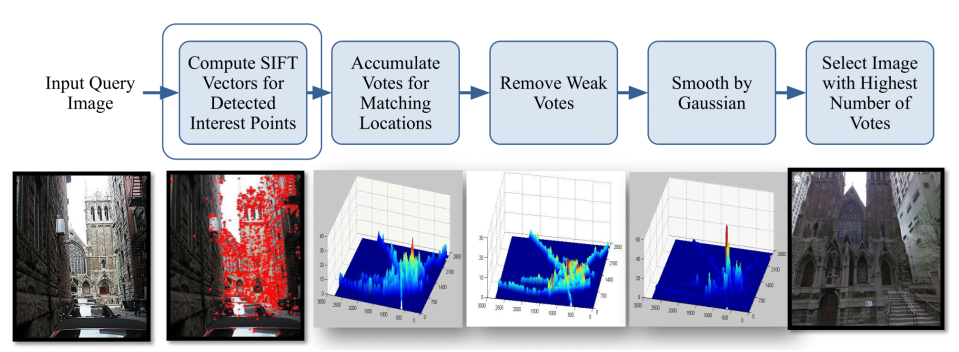
\includegraphics[scale=0.5]{pics/Chapter3/SIFT.png}
  \caption{Quy trình của mô hình sử dụng SIFT để trích xuất đặc trưng cục bộ \cite{zamir2010accurate}}
  \label{fig:enter-label}
\end{figure}

Trong những phương pháp sử dụng những phương pháp trích xuất truyền thống trước đây như SIFT \cite{lowe2004distinctive} và SURF \cite{bay2006surf} những đặc trưng được định nghĩa một cách thủ công sẽ được lấy ra từ ảnh. Những đặc trưng này bao gồm đặc điểm bề mặt, đường nét, những điểm đặc trưng, không gian hình học đặc biệt. Khoảng cách giữa các hình trong không gian đặc trưng sẽ là tiêu chí đánh giá về độ tương đồng. Từ đó, một tập những ảnh có những đặc trưng cục bộ giống với ảnh truy vấn nhất sẽ được tìm thấy từ hệ cơ sở dữ liệu và có thể xác định vị trí chụp ảnh truy vấn từ đó \cite{pion2020benchmarking}
\subsubsection*{Tổng hợp đặc trưng cục bộ}
Các đặc trưng cục bộ có thể được tổng hợp một lần nữa để có thể tạo ra một đoạn mã hóa mới cho ảnh. Việc này được thực hiện nhằm thu nhỏ kích thước mã hóa của ảnh, so với khi dùng đặc trưng cục bộ và giúp làm giảm sức ảnh hưởng từ những chi tiết của những vật không cố định bên trong ảnh, như xe hơi, cây cối, người đi bộ,... nhằm hướng đến việc sinh ra những cách mã hóa hóa ảnh không bị thay đổi khi góc chụp, độ sáng hay bị che khuất bởi vật thể \cite{jegou2010aggregating}.

Một số phương pháp tổng hợp cổ điển đã được sử dụng bao gồm hướng tiếp cận bag-of-visual-words \cite{philbin2007object}, VLAD \cite{jegou2010aggregating}, vector Fischer \cite{jegou2011aggregating}.

Với sự phát triển của công nghệ học sâu, các mạng neuron đã được ứng dụng vào cho việc trích xuất các đặc trưng của ảnh và đã có sự cải thiện rõ rệt về hiệu quả \cite{sunderhauf2015performance} so với cách trích xuất truyền thống
\subsubsection*{Ứng dụng của mạng neuron}

Với sự xuất hiện của mạng neuron, đặc biệt là mạng neuron tích chập, các tác vụ trích xuất và tổng hợp đặc trưng cục bộ của ảnh có thể được thực hiện mà không cần con người định nghĩa sẵn những quy luật nào.

Với việc trích xuất đặc trưng cục bộ, một bản đồ đặc trưng có thể được tạo ra từ việc chạy một ảnh qua một mô hình mạng neuron đã được huấn luyện. Tiếp theo đó, việc tổng hợp các đặc trưng này có thể được thực hiện bởi những lớp tiếp theo của mạng neuron tích chập, hoặc những phương pháp được truyền cảm hứng từ những phương pháp tổng hợp truyền thống. Do việc trích xuất và tổng hợp đặc trưng được thực hiện cùng trong một lần ảnh chạy qua mô hình, nên cơ chế này được gọi là detect-and-describe, khác với những phương pháp truyền thống là detect-then-describe \cite{9373578}

Một mạng neuron tích chập bình thường có thể được dùng cho mục đích trích xuất. Tuy nhiên, để có hiệu quả cao và tiết kiệm thời gian huấn luyện cho mô hình, các mô hình đã được huấn luyện sẵn sẽ được sử dụng như VGG, Res-Net, EfficientNet,... và bản đồ đặc trưng sẽ được lấy từ một lần truyền qua một mạng cơ sở đã được loại bỏ lớp cuối cùng.

Sau đó, ở bước tổng hợp, một số các lớp phương pháp đã xuất hiện như:
\begin{itemize}
  \item Một số phương pháp sẽ lấy cảm hứng từ những cách truyền thống, nhưng được điều chỉnh để trở thành một mạng huấn luyện được, như NetVLAD \cite{arandjelovic2016netvlad}, SPE-VLAD \cite{yu2019spatial}.
  \item Một lớp các phương pháp sẽ tập trung vào việc sử dụng một lớp tổng hợp - pooling layer để tổng hợp. Các phương pháp phổ biến bao gồm GeM \cite{radenovic2018fine}, MAC, R-MAC \cite{tolias2015particular}
\end{itemize}

\begin{figure}[H]
  \centering
  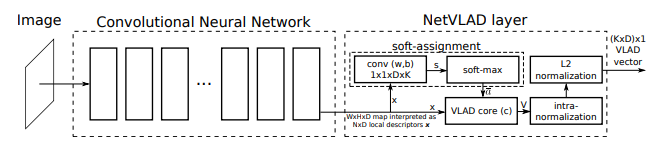
\includegraphics[scale=0.8]{pics/Chapter3/netvlad.png}
  \caption{Mô hình mã hóa ảnh bằng đặc trưng được truy xuất từ CNN và  NetVLAD \cite{arandjelovic2016netvlad}}
  \label{fig:enter-label}
\end{figure}

Trong thời gian gần đây, với sự phát triển của mô hình Transformer \cite{vaswani2023attention}, rất nhiều nghiên cứu đã hướng đến việc áp dụng mô hình này lên lĩnh vực trích xuất đặc trưng mã hóa ảnh cho bài toán truy xuất ảnh như AnyLoc \cite{keetha2023anyloc}, TransVPR \cite{wang2022transvpr}. Những hướng đi này đều đạt kết quả khả quan, tuy nhiên khả năng biểu diễn cho hình ảnh vẫn chưa thể vượt qua được NetVLAD \cite{alibey2023mixvpr}.

Với những tiến bộ trong mạng thần kinh đẳng hướng gần đây, cơ chế tự tập trung đã được chứng minh là không quá quan trọng cho những Vision Transformer \cite{dosovitskiy2021image}. Một minh chứng cho việc này chính là mô hình MLP-Mixer \cite{tolstikhin2021mlpmixer}, có cấu trúc chỉ gồm những lớp Perceptron. Mô hình này đã có kết quả cạnh tranh trong những tác vụ cơ bản của lĩnh vực thị giác máy tính.

\subsection{MLP-Mixer}
\subsubsection*{Định nghĩa}
Mạng MLP-Mixer, khác hẳn với những cấu trúc phức tạp như xu hướng của lĩnh vực học sâu trong thời gian gần đây, được cấu tạo hoàn toàn từ những lớp Perceptron. Vì vậy nên, các thao tác được thực hiện trong một lần xử lý ảnh chỉ bao gồm tác vụ nhân ma trận, thêm yếu tố phi tuyến tính vào mô hình và thay đổi bố cục của dữ liệu(nghịch đảo, thay đổi số chiều của ma trận).

Mạng MLP-Mixer sẽ nhận đầu vào là một ảnh. Ảnh này sau đó sẽ được cắt thành các mảnh không trùng lấp với nhau. Những mảnh này sẽ được tham chiếu lên một chiều không gian khác, gọi là không gian $C$, được thể hiện bằng một vector 1 chiều. Mỗi vector sẽ được gọi là một token và tập hợp các phần tử nằm ở cùng vị trí trên không gian $C$ ở mỗi vector sẽ được gọi là một kênh dữ liệu.

Mạng MLP-Mixer hoạt động dựa trên 2 cơ chế chính là pha trộn tokens và pha trộn theo kênh dữ liệu.
\begin{itemize}
  \item Pha trộn tokens - Tokens mixing sẽ giúp cho dữ liệu trên cùng một kênh có thể biết và tác động đến nhau. Cơ chế pha trộn tokens sẽ được thực hiện trên từng kênh dữ liệu một.
  \item Pha trộn theo kênh dữ liệu - Channel mixing giúp cho các dữ liệu nằm trên cùng một token có thể tác động lẫn nhau. Cơ chế pha trộn theo kênh sẽ được thực hiện trên từng token một.
\end{itemize}

\subsubsection*{Thực hiện}
Mạng Mixer sẽ nhận đầu vào là một ảnh đã được phân thành $S$ mảnh không trùng nhau. Từng mảnh sẽ có dạng dữ liệu là ma trận 2D sẽ được tham chiếu đến một chiều không gian $R^{C}$ và chuyển thành một vector 1 chiều có $C$ phần tử. Ma trận được dùng để tham chiếu sẽ được dùng chung cho quá trình chuyển đổi. Thông số $S$, số lượng những mảnh có kích thước $(P,P)$ của một ảnh có độ phân giải $(H,W)$ sẽ được tính bằng công thức:
$$
  S = \frac{H*W}{P^{2}}
$$

Sau đó các vector đại diện cho từng mảnh sẽ được nối lại với nhau, tạo thành một ma trận 2 chiều có dạng $R^{SxC}$. Với các hàng là những token(mã hóa của từng mảnh được cắt từ ảnh) và các cột là những kênh dữ liệu trên không gian $C$. Ma trận 2 chiều này sẽ được ký hiệu là $X$.

\begin{figure}[H]
  \centering
  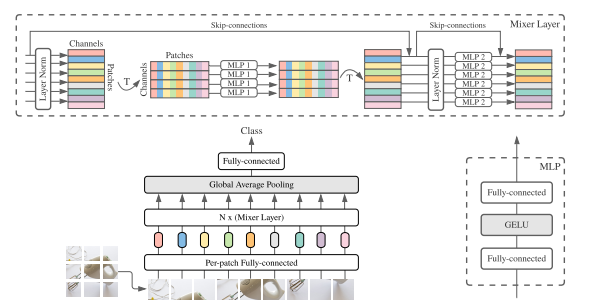
\includegraphics{pics/Chapter3/mixer.png}
  \caption{Cấu trúc của mô hình MLP-Mixer \cite{tolstikhin2021mlpmixer}}
  \label{fig:enter-label}
\end{figure}

Ma trận này sau đó sẽ được đưa qua những lớp Mixer, lần lượt pha trộn thông tin giữa các token và giữa các kênh dữ liệu.
\begin{itemize}
  \item Pha trộn tokens - Token mixing: Mạng MLP dành cho token-mixing sẽ được sử dụng để chiếu $R^{S}\rightarrow R^{S}$. Đối tượng thực hiện sẽ là các cột của $X$, là thông tin của một kênh dữ liệu trên những token.
  \item Pha trộn kênh dữ liệu - Channel mixing: Mạng MLP dành cho channel-mixing sẽ được sử dụng trên các hàng của $X$, gồm giá tri của các kênh trên từng token một. Mạng MLP này sẽ tham chiếu $R^{C}\rightarrow R^{C}$
\end{itemize}

Mỗi lớp MLP được sử dụng bên trong mô hình sẽ được cấu tạo từ 2 lớp mạng kết nối đầy đủ. Giữa lớp mạng đầu tiên và lớp mạng thứ hai, một lớp hàm kích hoạt sẽ được dùng để tạo sự phi tuyến tính cho quá trình. Ngoài ra, đầu vào của các mạng MLP đều sẽ được chạy qua một lớp chuẩn hóa và mỗi lần chạy qua một lớp MLP đều sẽ được kết nối tắt với giá trị ban đầu. Các công thức bên dưới sẽ tóm tắt được quá trình xử lý của một lớp mạng Mixer

$$
  U_*,i = X_*,i + W_2*\sigma(W_1*LayerNorm(X)_*,i),
$$
$$
  Y_j,* = U_j,* + W_4*\sigma(W_3*LayerNorm(U)_j,*)
$$
với $i = [1...C]$ và $j = [1...S]$. $\sigma$ là hàm không tuyến tính, trong bài báo này sẽ là hàm GELU \cite{hendrycks2023gaussian}.

Cuối cùng, dữ liệu sẽ được đưa vào một lớp tổng hợp trung bình toàn cục và qua một mạng kết nối đầy đủ trước khi trả về kết quả là một đoạn mã hóa cho ảnh đầu vào.

\subsubsection*{Đánh giá với các mô hình học sâu trước đây}
Về độ phức tạp khi tính toán, do các hàm pha trộn tokens và pha trộn kênh dữ liệu đều là những mô hình MLP vậy nên độ phức tạp của quá trình tính toán sẽ phát triển tuyến tính với số token và độ phân giải của hình. Cụ thể hơn, do độ rộng của các lớp bên trong mô hình MLP của mạng pha trộn tokens được định nghĩa không phụ thuộc vào số lượng các mảnh đầu vào, $S$, nên độ phức tạp tính toán sẽ phát triển tuyến tính với số lượng mảnh, khác với những mô hình Vision Transformer với độ phức tạp bậc hai. Độ rộng của các mô hình MLP pha trộn theo kênh cũng được chọn không phụ thuộc vào số lượng channel trong một mảnh, $C$, vậy nên độ phức tạp cũng sẽ tăng tuyến tính theo độ phân giải của ảnh, giống như một mạng neuron tích chập.

Một mô hình MLP dùng cho pha trộn các tokens sẽ được áp dụng cho mọi kênh dữ liệu và một mô hình MLP dùng để pha trộn các kênh trong một tokens cũng sẽ được dùng chung cho mọi tokens. Việc dùng chung một mạng MLP cho các kênh trong một tokens là một quyết định bình thường, nhằm giữ lại sự bất biến về vị trí trong ảnh, một yếu tố quan trọng trong mạng neuron tích chập. Tuy nhiên, việc sử dụng chung một mạng MLP nhằm pha trộn tokens cho các kênh dữ liệu thì ít phổ biến hơn. Tuy nhiên, việc sử dụng chung các thông số sẽ giúp giảm tốc độ tăng trưởng và tiết kiệm bộ nhớ của mô hình khi số mảnh $S$ hoặc số chiều của không gian $C$ tăng lên.

Mỗi lớp Mixer sẽ nhận đầu vào có kích thước không đổi. Kiến trúc này có những nét tương đồng với mạng Transformer hoặc những mô hình RNN trong những lĩnh vực khác. Đây là điểm khác biệt lớn với những mạng neuron tích chập khác, khi mà độ phân giải của đầu vào ở những lớp sâu hơn sẽ thấp, nhưng số kênh dữ liệu tăng lên.


\section{Kiến thức phương pháp ước tính vị trí của máy ảnh bằng Essential Matrix}
\subsection{Máy ảnh lỗ kim - Pinhole Camera}
Máy ảnh đo cường độ ánh sáng được chiếu đến nó bằng một con chíp. Bề mặt của chíp sẽ gồm nhiều khu vực và mỗi khu vực sẽ đo cường độ ánh sáng bằng cách đếm số photon đến được bề mặt của chíp. Lens của máy ảnh sẽ điều hướng ánh sáng đến được máy ảnh lên chíp và ảnh sẽ được tạo ra dựa trên lượng ánh sáng được điều đến các khu vực trên máy ảnh. Vậy nên, máy ảnh chỉ đo được lượng ánh sáng tới từ một hướng của một khu vực tới máy ảnh.


\subsection{Essential Matrix - Essential Matrix}
\subsection{Tìm sự tương ứng giữa đặc trưng ảnh - Feature Matching}
\subsection{Giải thuật 5 điểm ảnh - 5-Point Solver}
\subsection{Thuật toán tính độ sâu ảnh qua một ảnh - Monocular Depth Estimation}
\section{Sự liên kết giữa mô hình truy xuất ảnh và mô hình hồi quy tương đối}
Mặc dù có nhiều cách để thực hiện việc hồi quy ra vị trí ảnh:
\begin{itemize}
  \item Hồi quy dựa trên bản đổ đám mây điểm 3D toàn cục
  \item Hồi quy dựa trên bản đồ đám mây điểm 3D cục bộ
  \item Hồi quy dựa trên vị trí của các ảnh được truy xuất
\end{itemize}
Đa số các mô hình đều sử dụng cùng một cách biểu diễn khu vực, dựa trên những đặc trưng đã được thu gọn trên hình. Những đặc trưng này thường sẽ được huấn luyện cho những bài toán truy xuất địa danh, nhận diện khu vực. Vậy nên các đặc trưng này sẽ có những giá trị giống nhau khi các ảnh cùng nhìn một tòa nhà, một địa danh, kể cả dưới những góc nhìn khác nhau. Vậy nên, có thể kết quả của một mô hình thực hiện cả 2 tác vụ rời rạc này sẽ không đạt được kết quả tối ưu.\cite{pion2020benchmarking}

\textbf{Lưu ý:} Liệt kê ra những yêu cầu về đặc trưng cho những phương pháp khác nhau ở trên, cũng trong bài \cite{pion2020benchmarking}
\section{Tìm hiểu giới hạn của mô hình hồi quy vị trí tuyệt đối dựa trên mạng neuron tích chập}
Các mô hình hồi quy vị trí tuyệt đối sẽ xây dựng cách biểu diễn của khu vực trong tập dữ liệu một cách bao hàm. Thông qua đó, một số địa điểm bên trong khu vực được biểu diễn bởi tập dữ liệu sẽ được ngầm chọn làm điểm mốc. Điều này dẫn đến việc khi được huấn luyện trên những tập dữ liệu có hạn chế về mặt không gian thì mô hình hồi quy vị trí tuyệt đối sẽ không thể nào tổng quát hóa ra những khu vực không có trong tập dữ liệu ban đầu được mà phải huấn luyện lại trên tập dữ liệu của khu vực đó.\cite{sattler2019understanding}

Điều tương tự cũng có thể xảy ra với hồi quy tư thế tương đối, khi mà những ảnh truy xuất được có vị trí không đủ tổng quát thì có thể ảnh hưởng xấu đến kết quả của quá trình hồi quy tư thế tương đối

\textbf{Lưu ý}: Cần ghi ra phương pháp, cấu trúc mô hình được sử dụng trong bài. Cấu trúc khá đơn giản nên có thể không tổng quát hóa được. Cần ghi thêm các thí nghiệm của người ta.

\section{Tìm hiểu giới hạn của một số tập dữ liệu}
Một số tập dữ liệu quá thưa, không phản ánh được chính xác vùng mà tập dữ liệu muốn miêu tả, mà nó dày quá thì mô hình chạy không nổi\cite{berton2022rethinking}
